\documentclass[Master]{subfiles}
\begin{document}
\subsection{Topological Solid State Physics}
Topological Solid State Physics introduces a zoology on the space of Hamiltonians $\Xi$.
Hamiltonians are considered topologically equivalent $\sim_{(top)}$ when they can be connected without crossing a critical point or region. Thus, the spectrum remains gapped and no state band crosses zero. The adiabatic theorem \cite{born1928beweis} then guarantees that the ground state is an instantaneous eigenstate up to phase (more in \secref{anal:Adiabati}). 
Mathematically, this is described by the existence of a homotopy. Two Hamiltonians $H_1, H_2 \in \Xi$ are topologically equivalent exactly when there exists a continuous function $H(t)$:
$$ H_1 \sim_{(top)} H_2 \iff \forall t \in [0,1] \exists  \  H : [0,1] \rightarrow  \Xi, t \rightarrow H(t) :
H(t) = \begin{cases}
H_0 & t = 0 \\
H_1 & t = 1
\end{cases}
$$
$$\forall t \in [0,1] \nexists \ket{\phi} : H(t)\ket{\phi} = 0 $$
However, as many systems are not solvable analytically, finding such a homotopy becomes challenging. A more helpful approach is topological invariants.\\
Let $ f: \Xi \rightarrow \mathbb{S}, H \rightarrow f(H) $ with $\mathbb{S}$ some space:

$$f \ \text{is a topological invariant}  \iff  \forall H_1,H_2 \in \Xi: H_1 \sim_{(top)} H_2 , f(H_1) = f(H_2)$$
The converse does not generally hold:
$$
f(H_1) = f(H_2) \nRightarrow  H_1 \sim_{(top)} H_2 
$$
Thus, a homotopy can show topological equivalence whereas a topological invariant can only show a difference.

\subsubsection{Berry Phase}\label{sec:BerryPhase}
Given a Hamiltonian $H(\vec{R})$ depending on some parameter space $\vec{R} \in \mathbb{K}^{N}$ and a set of eigenstates $\ket{\phi(\vec{R})_i}$ such that $H(\vec{R})\ket{\phi(\vec{R})_i} = E_i(\vec{R})\ket{\phi(\vec{R})_i}$.
The adiabatic time evolution of the phase can be calculated as
$$
\theta_i(t) = \underbrace{\frac{1}{\hbar}\int_{0}^{t} E_i(\vec{R(t')}) dt'}_{Dynamical Phase} - \underbrace{i \int_{0}^{t} \bra{\phi(\vec{R(t)})_i} \frac{d}{dt}\ket{\phi(\vec{R(t)})_i}}_{Berry Phase} + \theta_i(0)
$$
The phase is split between dynamical and Berry phase. While the Berry phase is gauge dependent on a general trajectory through $\mathbb{K}^{N}$ the phase on a closed loop is gauge independent:
$$
\gamma_i = - \Im \oint dS_l \epsilon_{ljk} \braket{\nabla_j \phi_n(\vec{R})}{\nabla_k \phi_n(\vec{R})}
$$
$$= - \Im \oint dS_l \epsilon_{ljk}  \sum_m \frac{ \bra{\phi_i(\vec{R})}\nabla_j H \ket{\phi_m(\vec{R})}
\bra{\phi_m(\vec{R})}\nabla_k H \ket{\phi_i(\vec{R})}}{(E_k-E_j)^2}
$$ Furthermore the closed Loop Berry curvature is a topological invariant.
An illustrative example is the case of a Berry curvature of $\pi$ on some closed path $\mathcal{C}$.
One can illustratively imagine a torus $[0,2 \pi] \times \mathcal{C}$ with phase being the minor radius and $\mathcal{C}$ being the major radius. The Berry phase turns by $\pi$ around the minor radius for every $2\pi$ rotation around the major radius. Only after two revelations does the phase return to its origin on the torus.
This time evolution encloses a Mobius strip contrary to a Berry phase of $0$ which is simply a circle.  While a gauge transformation may deform the phase continuously on the torus it cannot transform the perimeter of a Mobius strip into a simple circle. The two Berry phases are topologically different. 
\begin{figure}[H]
    \centering
    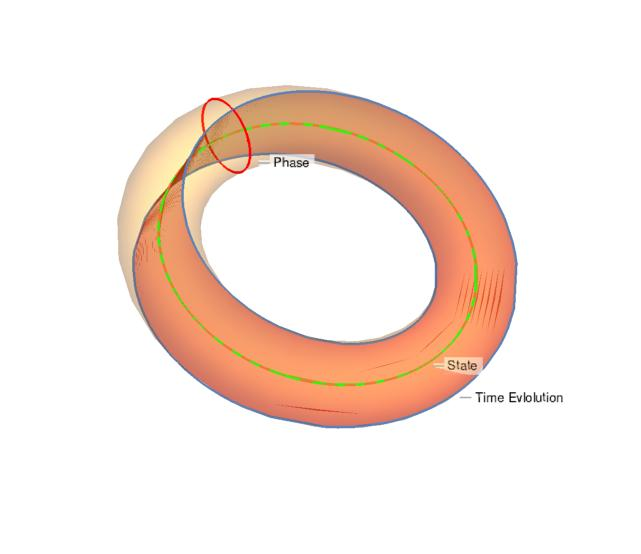
\includegraphics[width=0.5\linewidth]{imgs/TopPhseTorus.jpeg}
    \caption{Adiabatic Time evolution on a symbolic torus "State $\times$  Phase".
    The Berry phase wraps around the torus enclosing a Mobius strip.
    }
    \label{fig:my_label}
\end{figure}
When the state is degenerate the non-abelian Zack-Wilczek phase \cite{wilczek1984appearance} occurs,
where a time-dependent unitary matrix acts on the degenerate states.
\subsubsection{Classification}
The necessary topological invariants to classify a Hamiltonian $H$ can be deduced from the spacial dimension and the presence of time reversal $\mathcal{T}$, charge conjugation $\mathcal{C}$ and chiral $\mathcal{S}$ symmetry analogous to \cite{ryu2010topological}: 
$$
\mathcal{T}H = H^*\mathcal{T}
$$
$$
\mathcal{C}H = -H^*\mathcal{C}
$$
$$
\mathcal{S}H = -H\mathcal{S}
$$ 
The time reversal and charge conjugation symmetry are both antiunitary symmetries and either square to plus or minus the identity:
$$\mathcal{T}^2=\pm \mathbb{1}; \ \mathcal{C}^2= \pm \mathbb{1}$$
The chiral symmetry is unitary and can only be present when both $\mathcal{T}$ and $\mathcal{C}$ are either both present or not. Given a $\mathcal{T}$ and $ \mathcal{C}$ symmetry the $\mathcal{S}$ symmetry can be represented as the product of the two:
$$\mathcal{C}\mathcal{T}=\mathcal{S}$$
A chiral symmetry allways squares to identity $\mathcal{S}^2 = \mathbb{1}$. Thus there are 10 possible cases.
Given the presence of these symmetries the Cartan classification can be deduced from \figref{fig:10FoldWay}.
\begin{figure}[H]
    \centering
    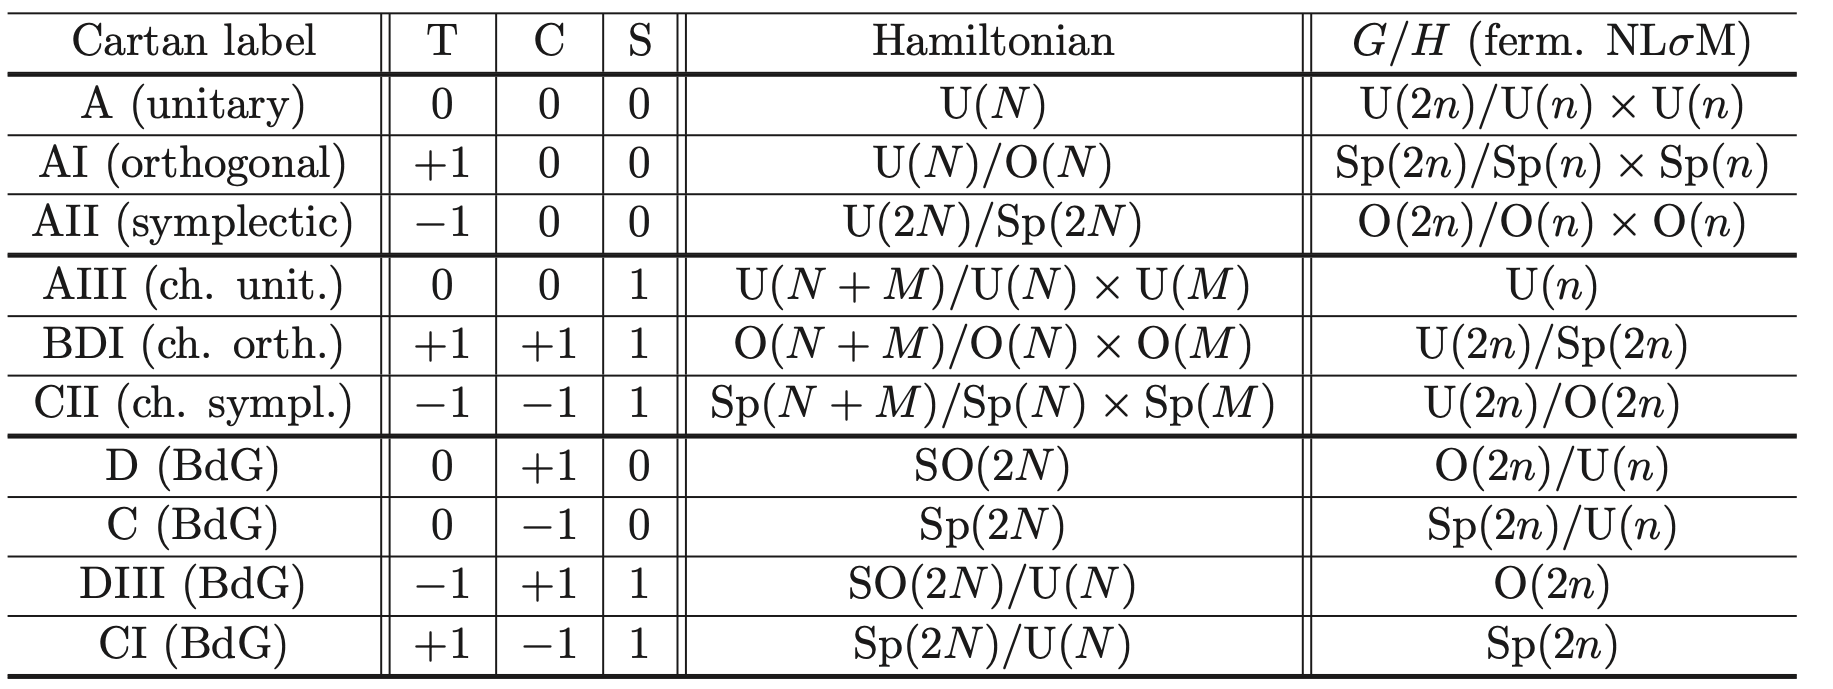
\includegraphics[width=\linewidth]{imgs/10FoldWay.png}
    \caption{Cartan random matrix classification / The 10 fold way from \cite{ryu2010topological}}
    \label{fig:10FoldWay}
\end{figure}
In combination with the dimension the class of topological invariant $\mathbb{Z},\mathbb{Z}_2$ or $2\mathbb{Z}$ can be deduced from \figref{fig:TopInvariants}.
\begin{figure}[H]
    \centering
    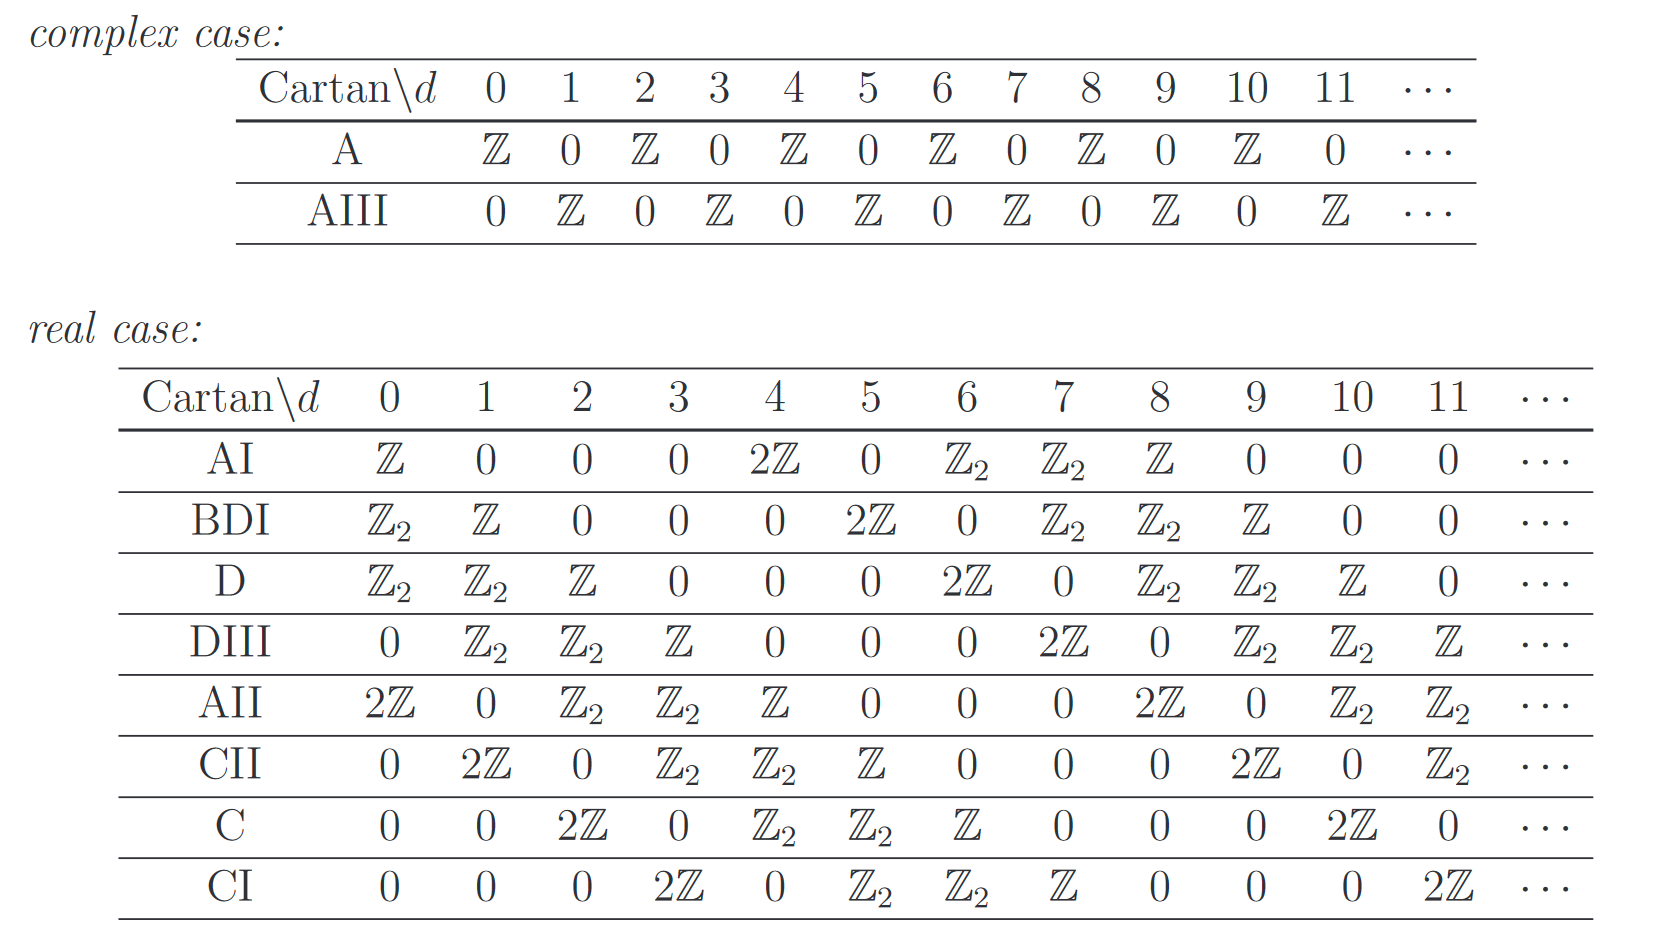
\includegraphics[width=\linewidth]{imgs/TopInvariants.png}
    \caption{Types of topological invariants from \cite{ryu2010topological}}
    \label{fig:TopInvariants}
\end{figure}
further details in \cite{ryu2010topological}.

\subsubsection{Edge Bulk Correspondence}\label{sec:BulkEdgeCorrespondance}
When two topologically different bulk materials share a boundary, zero energy edge states can occur. The existence of edge states depends on the dimension of the interface, and the topological classification of the bulk materials surrounding it \cite{teo2010topological}. For example, in a one-dimensional topological superconductor of D class, an interface between two topologically distinct sections is a point, and a Majorana mode can occur see \figref{fig:TopPointDefect}. In two dimensions, the simplest interface between two topologically distinct sections is a line. Here a chiral Majorana mode can occur see \figref{fig:TopLineDefects}. In a topological insulator, these gapless modes can give rise to edge conductivity\cite{volkov1985two}.
\begin{figure}[H]
    \centering
    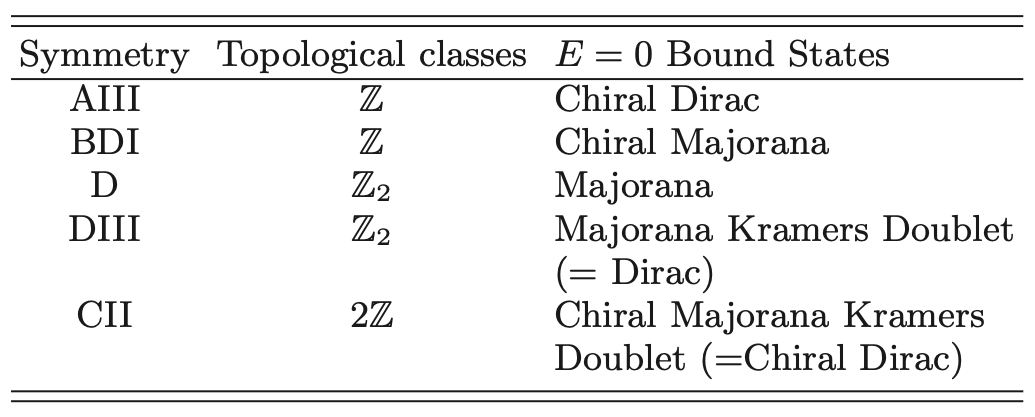
\includegraphics[width=0.7\textwidth]{imgs/TopPointDefect.png}
    \caption{Zero-ernergy modes on Point interfaces and respective Symmetry classes.
    Figure adapted from \cite{teo2010topological}}
    \label{fig:TopPointDefect}
\end{figure}
\begin{figure}[H]
    \centering
    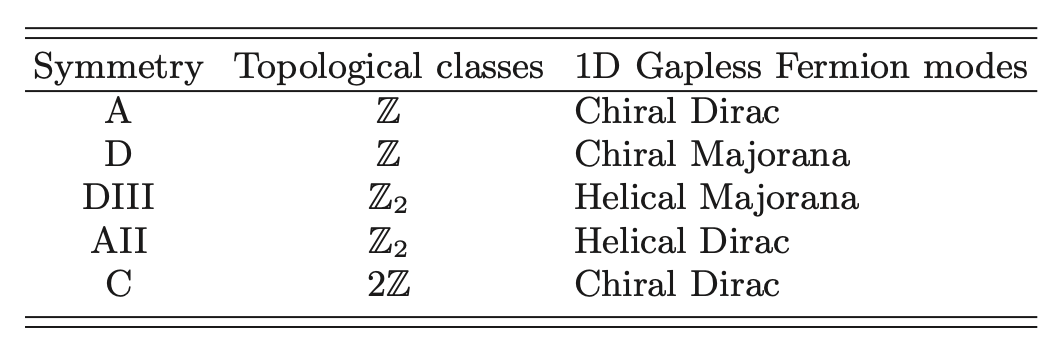
\includegraphics[width=0.7\textwidth]{imgs/TopLineDefect.png}
    \caption{Zero-ernergy modes on Line interfaces and respective Symmetry classes.
    Figure adapted from \cite{teo2010topological}}
    \label{fig:TopLineDefects}
\end{figure}


\end{document}